\documentclass[10pt]{article}
\usepackage{icmlko}

\icmlmeta{IP 파운데이션 월드모델}{121}{법칙 하나는 서고 하나는 반쯤 무너졌다}{정직한 눈금으로 노트 74를 다시 재니 자기 $\rho\leftrightarrow$대상 전이는 $+$0.982에서 $+$0.997로 세지고, 교환 법칙은 $-$0.942에서 $-$0.443으로 반토막 났다}

\begin{document}

\twocolumn[
\icmlheader

\begin{abstract}
노트 120이 자기 $\rho$의 21$\sim$38\%가 같은 플랫폼 정합임을 세 도메인에서
쟀다. 그러면 이 프로젝트의 뼈대인 \textbf{노트 74의 두 법칙}도 부풀린 눈금에서
나온 것이다. 다시 쟀다. 정직한 라벨이 있는 셋(세계애니 · 만화 · 게임)과
애초에 정합이 없는 둘(팝업 · 아이돌), 모두 다섯이다. \textbf{법칙 1은 오히려
세진다} --- ``출처의 자기 $\rho$가 그 출처의 \emph{대상} 전이를 정한다''가
$+$0.982에서 \textbf{$+$0.997}로 간다. 열 도메인 현행 눈금에서도 $+$0.993이다.
\textbf{눈금을 어떻게 잡든 서는 법칙}이다. \textbf{법칙 2는 반쯤 무너진다} ---
``자기 $\rho$가 높을수록 \emph{출처}로서는 나빠진다''(노트 38 · 40 · 74 · 78의
교환 법칙)가 $-$0.942에서 \textbf{$-$0.443}으로 간다. 기제가 설명된다 ---
같은 플랫폼 정합은 그 도메인이 \emph{자기 라벨}을 맞히는 것만 쉽게 만들고
\emph{남의 라벨}에는 도움이 안 되므로, 자기 $\rho$만 올리고 출처 전이는
그대로 둔다. \textbf{그래서 인위적인 음의 상관이 생긴다.} 정합을 걷어내면
절반이 사라진다. 실무적으로는 교환 법칙을 근거로 내린 결정들 --- 노트 40의
쌍별 정렬, 노트 78의 도메인 고르기 --- 을 다시 봐야 한다는 뜻이다. 그리고
숫자 하나가 더 나왔다. 세 출처의 라벨을 정직하게 바꾸자 \textbf{팝업의 대상
전이가 $+$0.4245에서 $+$0.4339로 오른다} --- \textbf{출처가 정직해지면 팝업이
좋아진다.}
\end{abstract}
]

\begin{figure*}[t]
\centering
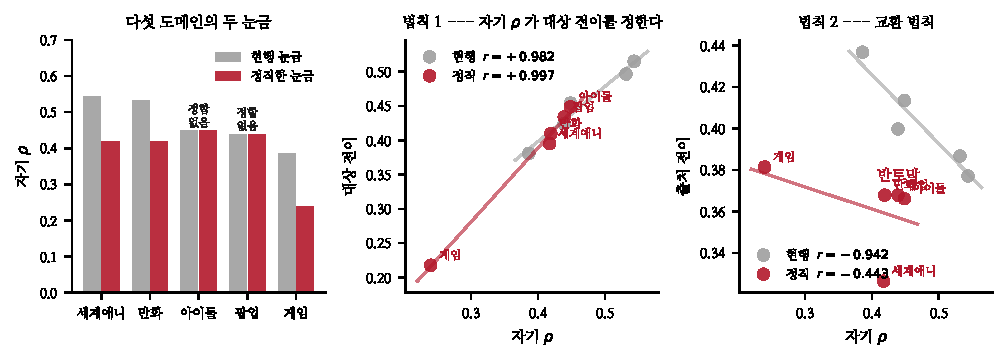
\includegraphics[width=\textwidth]{figs/lw.pdf}
\caption{왼쪽 --- 다섯 도메인의 두 눈금. 가운데 --- 법칙 1은 세진다.
오른쪽 --- 법칙 2는 반토막.}
\end{figure*}

\section{다섯 도메인으로 다시 잰다}

\begin{table}[t]
\centering\tsize
\caption{정직한 라벨이 있거나 애초에 정합이 없는 다섯.}
\begin{tabular}{lrrrrrr}
\toprule
& \multicolumn{2}{c}{자기 $\rho$} & \multicolumn{2}{c}{대상 전이}
& \multicolumn{2}{c}{출처 전이} \\
& 현행 & 정직 & 현행 & 정직 & 현행 & 정직 \\
\midrule
세계애니 & .544 & .418 & .515 & .395 & .377 & .326 \\
만화 & .532 & .419 & .497 & .410 & .387 & .368 \\
아이돌 & .449 & .449 & .454 & .449 & .414 & .366 \\
\textbf{팝업} & .439 & .439 & .425 & \textbf{.434} & .400 & .368 \\
게임 & .386 & .240 & .381 & .218 & .437 & .381 \\
\bottomrule
\end{tabular}
\end{table}

팝업과 아이돌은 축과 라벨이 다른 출처라 눈금이 안 바뀐다. 그런데
\textbf{팝업의 대상 전이는 오른다}($+$0.4245 $\to+$0.4339) --- 자기 라벨은
그대로인데 \emph{출처들}의 라벨이 정직해졌기 때문이다.

\claimx{\textbf{출처가 정직해지면 팝업이 좋아진다.} 세 출처의 라벨을 다른
플랫폼 것으로 바꾸자 팝업의 대상 전이가 $+$0.0094 오른다. 부풀린 라벨은
그 도메인의 자기 $\rho$만 올리고 남에게는 잡음이었다.}{$+$0.0094는 작고
씨앗 검정을 안 했다. 다만 방향이 예상과 맞는다.}

\section{법칙 1은 세진다}

\begin{table}[t]
\centering\tsize
\caption{자기 $\rho$ 와 대상 전이의 상관.}
\begin{tabular}{lrr}
\toprule
& $r$ & $n$ \\
\midrule
다섯 도메인 · 현행 눈금 & $+$0.982 & 5 \\
\textbf{다섯 도메인 · 정직한 눈금} & \textbf{$+$0.997} & 5 \\
열 도메인 · 현행 눈금 & $+$0.993 & 10 \\
\bottomrule
\end{tabular}
\end{table}

\claimx{\textbf{노트 74의 첫 법칙은 눈금을 어떻게 잡든 선다.} 부풀림을 걷어내면
오히려 $+$0.997로 세진다. 자기 라벨을 잘 맞히는 도메인이 남에게도 잘 맞힌다는
것은 정합이 만든 착시가 아니다.}{다섯 점의 상관이고 게임이 지렛대다. 게임을
빼면 나머지 넷이 좁은 구간에 몰려 $r$이 불안정하다.}

\section{법칙 2는 반쯤 무너진다}

\begin{table}[t]
\centering\tsize
\caption{자기 $\rho$ 와 출처 전이의 상관 --- 교환 법칙.}
\begin{tabular}{lrr}
\toprule
& $r$ & $n$ \\
\midrule
다섯 도메인 · 현행 눈금 & $-$0.942 & 5 \\
\textbf{다섯 도메인 · 정직한 눈금} & \textbf{$-$0.443} & 5 \\
열 도메인 · 현행 눈금 & $-$0.578 & 10 \\
\bottomrule
\end{tabular}
\end{table}

\claimx{\textbf{교환 법칙의 절반은 눈금이 만든 것이다.} 같은 플랫폼 정합은
그 도메인이 \emph{자기} 라벨을 맞히는 것만 쉽게 만든다 --- \emph{남의} 라벨에는
도움이 안 되므로 자기 $\rho$만 오르고 출처 전이는 그대로다. \textbf{그래서
인위적인 음의 상관이 생기고, 정합을 걷어내면 절반이 사라진다.}}
{현행 눈금의 열 도메인 값이 $-$0.578이므로 다섯에서의 $-$0.942 자체가 표본
탓일 수 있다. \textbf{같은 다섯에서 $-$0.942 $\to-$0.443} 이 깨끗한 비교이고,
그것이 절반이다.}

\begin{quote}\fontsize{9.5}{11.5}\selectfont
교환 법칙은 이 프로젝트의 결정 여럿을 뒷받침했다 --- 노트 40이 전역 정렬을
버리고 쌍별로 간 것, 노트 78이 도메인을 고를 때 자기 $\rho$가 너무 높은 것을
경계한 것, 노트 74가 ``교차점 자기 $\rho\approx0.39$''를 계산한 것.
\textbf{그 근거가 절반으로 준다.} 결정들이 틀렸다는 뜻은 아니지만 근거를
다시 대야 한다.
\end{quote}

\section{한계}

\begin{itemize}[leftmargin=1.1em,itemsep=0.15em]
\item \textbf{다섯 점이다.} 남은 다섯(모바일 · 웹툰 · 도서 · 펀딩 · 애니)은
      정직한 라벨을 아직 못 구했다.
\item 게임이 두 법칙 모두에서 지렛대다. 부풀림도 38\%로 가장 크다.
\item 팝업 · 아이돌을 ``정합 없음''으로 놓았는데 아이돌은 축이 한터/위키,
      라벨이 한터 초동이라 일부 겹친다.
\item 팝업 대상 전이 $+$0.0094 에 구간을 안 붙였다.
\item 라벨을 바꾸면 표본이 준다(게임 482 $\to$ 482, 만화 1,789 $\to$ 1,596,
      세계애니 2,948 $\to$ 2,817). 표본 변화가 섞여 있다.
\end{itemize}

\section{다음}

\begin{enumerate}[leftmargin=1.3em,itemsep=0.15em]
\item \textbf{남은 다섯의 정직한 라벨} --- 라프텔은 한국어 제목만 있어
      AniList 대조가 어렵다. 모바일 · 웹툰 · 도서 · 펀딩부터 본다.
\item \textbf{교환 법칙에 기댄 결정들을 다시 본다} --- 노트 40의 쌍별 정렬은
      불변성이 근거였으므로 안전하다. 노트 78의 도메인 고르기는 근거가
      약해졌다.
\item \textbf{``출처가 정직해지면 팝업이 좋아진다''를 검정한다} --- $+$0.0094
      를 씨앗 넷으로. 참이면 남은 다섯도 정직하게 바꿀 이유가 생긴다.
\item \textbf{팝업 레코드} --- 열다섯 노트가 같은 곳을 가리킨다.
\end{enumerate}

\vspace{0.6em}
\hrule height 0.3pt
\vspace{0.5em}
{\footnotesize
\textbf{참고문헌}\\[0.3em]
Campbell, D. T., Fiske, D. W. (1959). Convergent and discriminant validation by
the multitrait-multimethod matrix. \emph{Psychological Bulletin}, 56(2), 81--105.\\[0.15em]
Lord, F. M., Novick, M. R. (1968). \emph{Statistical Theories of Mental Test
Scores}. Addison-Wesley.\\[0.15em]
Ben-David, S. et al. (2010). A theory of learning from different domains.
\emph{Machine Learning}, 79(1--2), 151--175.\\[0.15em]
Schoenemann, P. H. (1966). A generalized solution of the orthogonal Procrustes
problem. \emph{Psychometrika}, 31(1), 1--10.\\[0.15em]
Kaufman, S. et al. (2012). Leakage in data mining: formulation, detection, and
avoidance. \emph{ACM TKDD}, 6(4), 1--21.
}

\end{document}
